\documentclass{article}

\usepackage{graphicx}
\usepackage{tikz}
\usetikzlibrary{calc, spy}
\usepackage{adjustbox}
\usepackage[tightpage, active, floats, graphics]{preview}
\usepackage{overpic}

\begin{document}
\begin{preview}
    \vspace{1cm}
    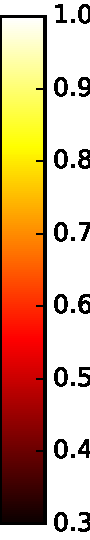
\includegraphics[width=.0335\linewidth]{scores_colorbar}
    %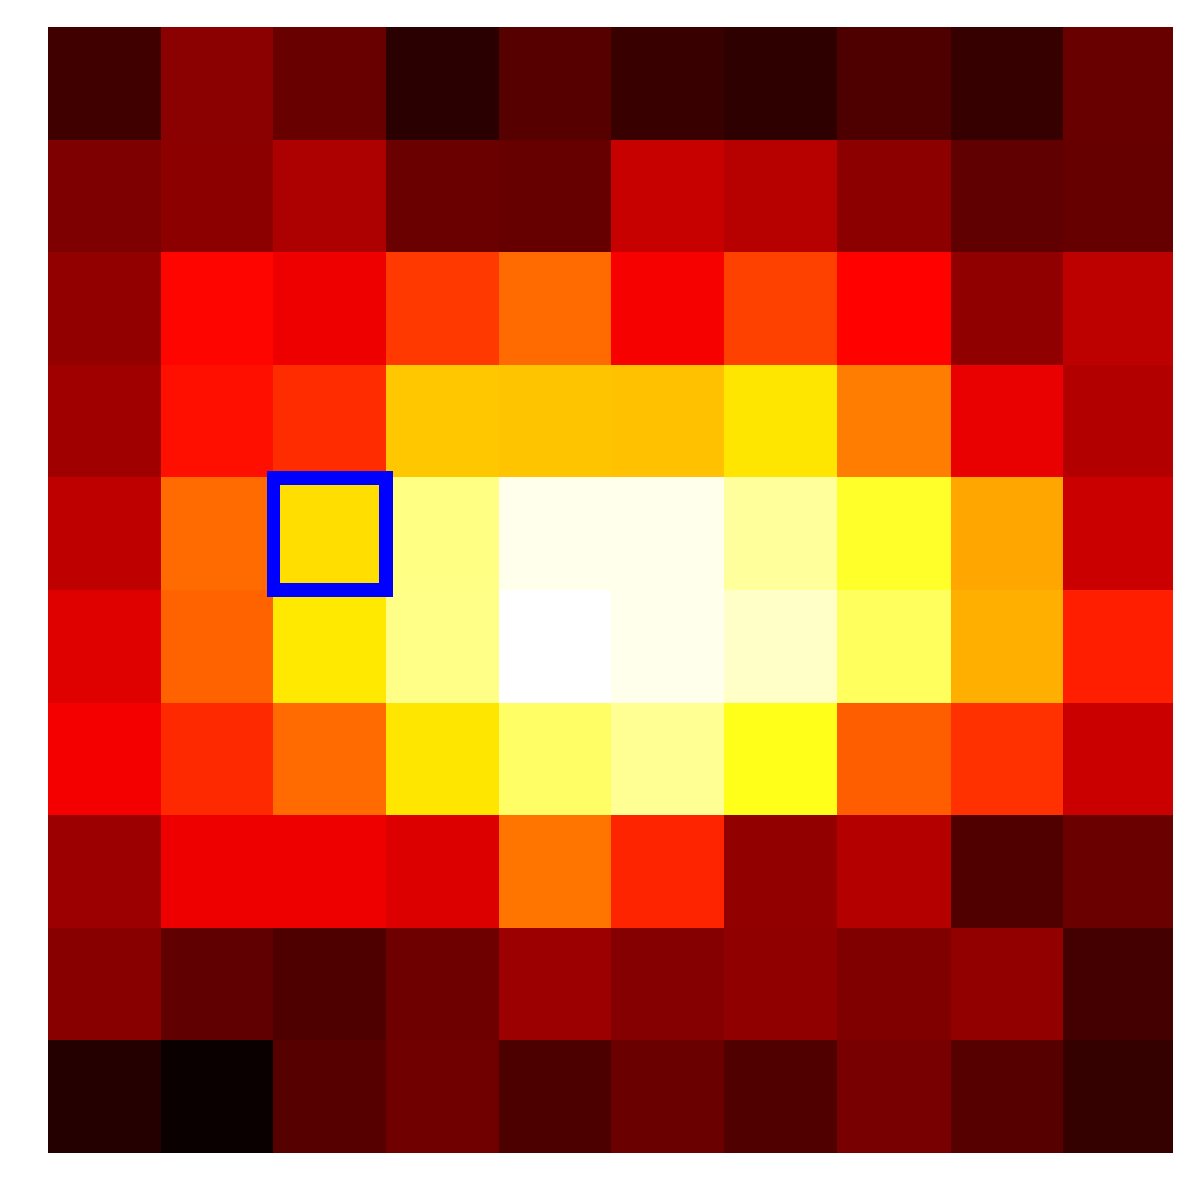
\includegraphics[width=\linewidth]{img/kamitani/scores_log}
        \begin{overpic}[width=.2\linewidth]{scores_log}
            \put(2, 2){\sffamily\bfseries a}
        \end{overpic}%
    %\subcaption{Logistic regression scores}
        \begin{tikzpicture}
          \begin{scope}[spy using outlines={blue, circle, line width=1pt,
                magnification=6, size=60, connect spies}]
            \node[inner sep=0pt, rotate=90](img){
                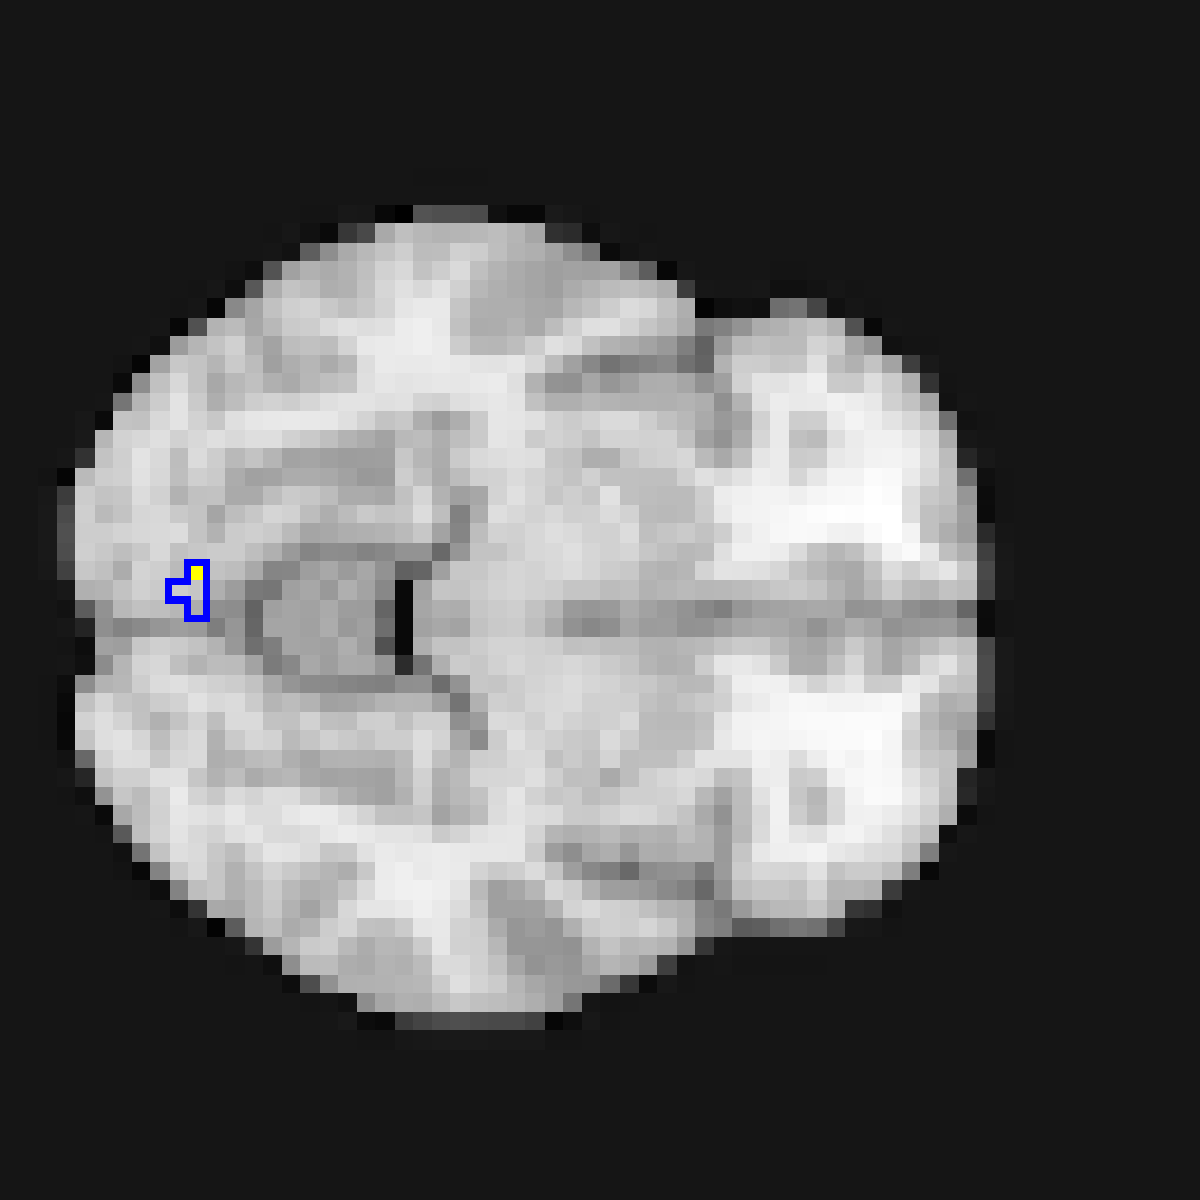
\includegraphics[width=.2\linewidth]{pixel_logistic}};
            \node[inner sep=0pt] at (-1., -1.)
		{\textcolor{white}{\sffamily\bfseries b}};
            \spy [width=1.5cm, height=1.5cm, line width=3pt, spy connection path={\draw[line
            width=2pt, blue] (tikzspyonnode) -- (tikzspyinnode);}]
            on (-0.02, -.82) in node (a) [line width=4pt] (a) at (.3, .3) (a) {};
        \end{scope}
    \end{tikzpicture}
        \begin{overpic}[width=.2\linewidth]{scores_svc}
            \put(2, 2){\sffamily\bfseries c}
        \end{overpic}%
        \begin{tikzpicture}
          \begin{scope}[spy using outlines={blue, circle, line width=1pt,
                magnification=6, size=60, connect spies}]
            \node[inner sep=0pt, rotate=90](img){
                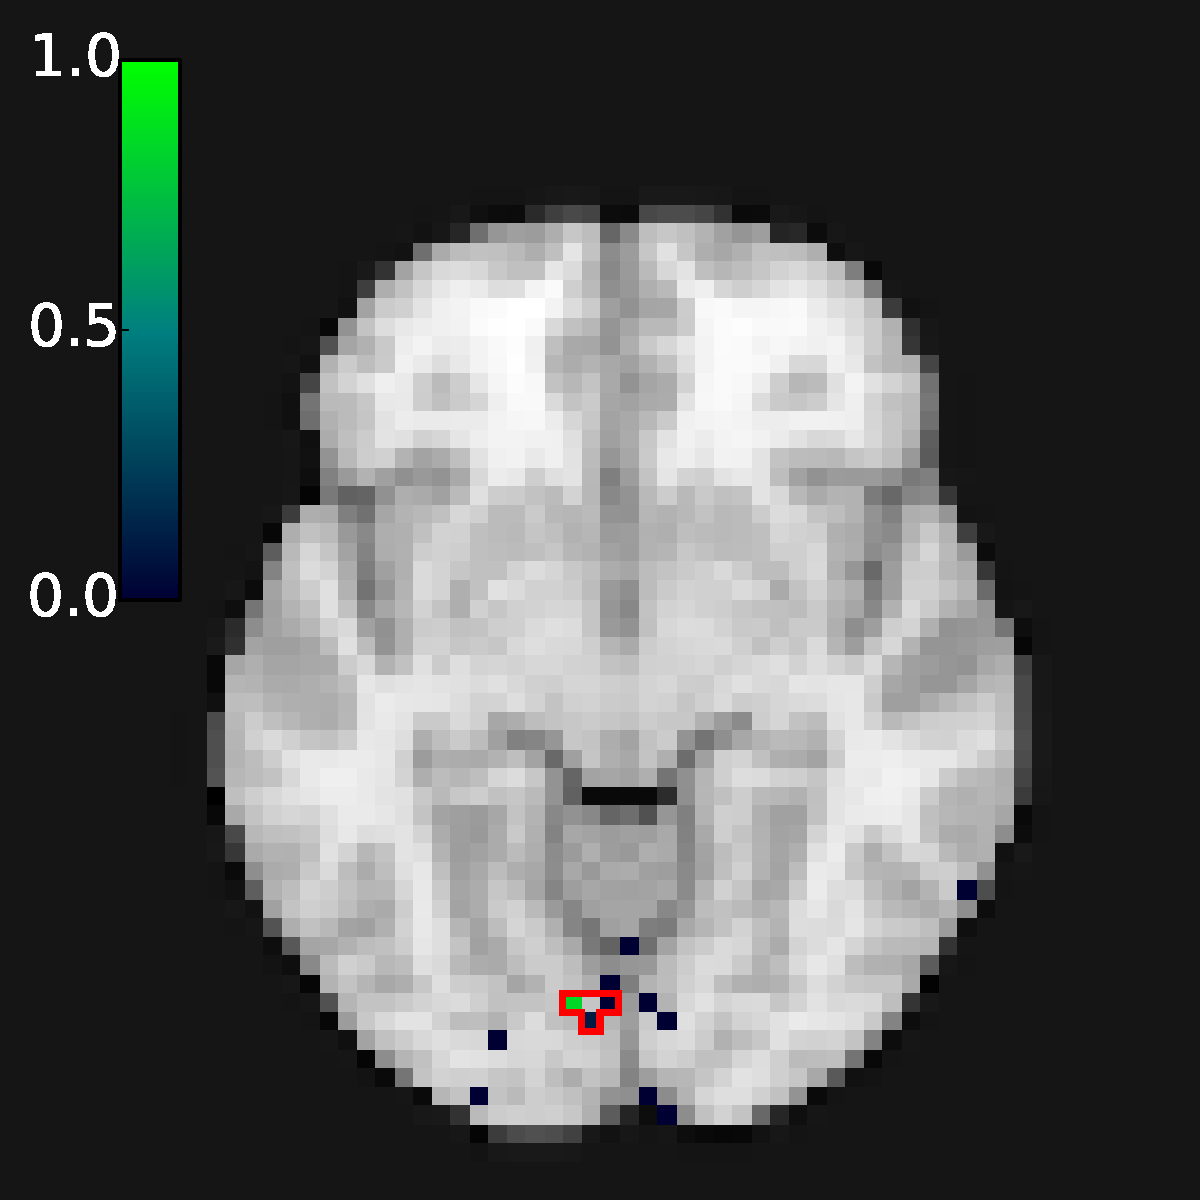
\includegraphics[width=.2\linewidth]{pixel_svc}};
            \node[inner sep=0pt] at (-1., -1.)
		{\textcolor{white}{\sffamily\bfseries d}};
            \spy [width=1.5cm, height=1.5cm, line width=3pt, spy connection path={\draw[line
            width=2pt, blue] (tikzspyonnode) -- (tikzspyinnode);}]
            on (-0.02, -.82) in node (a) [line width=4pt] (a) at (.3, .3) (a) {};
        \end{scope}
    \end{tikzpicture}
\end{preview}
\end{document}
